\documentclass[main.tex]{subfiles}
\begin{document}

General Instructions. Read carefully before starting. Solve 5 problems in all; at most 2 questions may be selected from the same section. Candidates registered in the following focus areas must answer two of their five questions from the relevant section as follows:\\

\begin{itemize}
    \item Computer Architecture and High-Performance Computing: Section 1
    \item Communications \& Networks: Section 3
    \item Electrical Power \& Energy: Section 8
    \item Electromagnetics, Radiation Systems \& Microwave Engineering: Section 4
    \item Electronics, Photonics \& MEMS: Section 6
    \item Signal \& Image Processing, Systems \& Controls: Section 3
\end{itemize}

Please write your name and student number below:\\\\

Solve each problem in a \underline{separate} blue book. Write the section number, problem number, and your student number on the front of each blue book. Do not write your name on the blue book. Submit solutions to only five \(5\) problems. Use only one blue book per problem. For each problem, make a special effort to give the answers in a clear form. The exam will begin at 10:00 a.m. and end promptly at 3:00 p.m. Only calculators provided by the department at the examination will be allowed. Personal items including cell phones and other electrical devices must be relinquished prior to the start of the examination. This is a closed book, closed notes examination.

\begin{enumerate}

\subsection{Section 1 Computer Architecture and High-Performance Computing}

\item Compiler performance can be quantified by execution time $T$ (Eq. \ref{eq:executionTime}) where $IC$ is the instruction count in a given program, $CPI$ is number of cycles per instruction, and $CT$ is the clock time. Additionally $CT=1/f$ where $f$ is the clock rate.

\begin{equation} \label{eq:executionTime}
T = IC \times CPI \times CT
\end{equation}

The un-optimized compilers clock rate is 15\% higher than the optimized version $\therefore f_{u} = 1.15f_{o}$. The cycle time for the optimized compiler is $\therefore CT_o = 1.15CT_u$. The un-optimized compiler instructions are comprised of 45\% loads and stores and the optimized compiler instructions, which is 1/3 of the un-optimized, are comprised of 15\% loads and stores. However since it is given that all instructions, including load and store, take one clock cycle the percent of loads and stores is irrelevant and $\therefore CPI_o = CPI_u$. For the same program the instruction count for the optimized and un-optimized compilers will remain the same $\therefore IC_o = IC_u$. Clock time is the only factor the differs between compilers and $\because CT_o > CT_u \therefore T_o > T_u$. An increase in execution time for the optimized compiler is a degradation in performance and therefore the un-optimized compiler is the faster version.

\item 
\begin{enumerate}
    \item The maximum normalized number that can be computed using single bit precision is comprised of the sign bit $b_{31} = 0$ with $S=0$, exponent bits $b_{30} b_{29} \cdots b_{24}$ set to 1 and $b_{23}$ set to 0, accounting for the exponent bit values of all zeros and all ones reserved for special numbers, with the $Exponent = \sum_{i=0}^{7} b_{23+i} 2^{+i} = 254$, and fraction bits $b_{22} b_{21} \cdots b_{0}$ set to 1 with the $Fraction = \sum_{i=1}^{23} b_{23-i} 2^{-i} \approx 0.999$, resulting in the calculation $(-1)^0 \times (1+0.999) \times 2^{(254-127)} = 1 \times 1.999 \times \num{1.7014118e38} \approx \num{3.401e38}$. 
    
    The absolute minimum normalized number that can be computed using single bit precision is comprised of the sign bit $b_{31} = 1$ with $S=1$, $Exponent$ and $Fraction$ that same as for the maximum calculation, and calculated as $(-1)^1 \times (1+0.999) \times 2^{(254-127)} = -1 \times 1.999 \times \num{1.701e38} \approx \num{-3.401e38}$.
    
    \item The (absolute) maximum denormalized single bit precision number is comprised of sign bit $b_{31} = 0$ or $b_{31} = 1$, exponent bits $b_{30} b_{29} \cdots b_{23}$ set to 0, and fraction bits $b_{22} b_{21} \cdots b_{0}$ set to 1 with value $\sum_{i=1}^{23} b_{23-i} 2^{-i} = (1-2^{-23})$, resulting in a calculated value (positive example) of $(-1)^0 \times (0+(1-2^{-23}) \times 2^{(1-127)} \approx \pm\num{1.18e-38}$. 
    
    The absolute minimum denormalized single bit precision number differs from the maximum with fraction bits $b_{22} b_{21} \cdots b_{1}$ set to 0 and $b_{0}$ set to 1 with value $\sum_{i=1}^{23} b_{23-i} 2^{-i} = 2^{-23}$ resulting in a calculated value (positive example) of $(-1)^0 \times 0+2^{-23} \times 2^{(1-127)} \approx \pm\num{1.4e-45}$.
    
    \item 
    \begin{enumerate}
        \item The original bias of 127 is half the maximum exponent value of 254, using that logic the new bias should equal $\frac{2^{10} - 2}{2} = \frac{1022}{2}=512$ 
        
        \item The absolute maximum normalized single bit precision number is comprised of sign bit $b_{31} = 0$ (positive example), exponent bits $b_{30} b_{29} \cdots b_{22}$ set to 1 and $b_{21}$ set to 0, accounting for all ones reserved for positive and negative infinity, with value $\sum_{i=0}^{9} b_{21+i} 2^{+i} = 1022$, and fraction bits $b_{20} b_{19} \cdots b_{0}$ set to 1 with value $\sum_{i=1}^{21} b_{21-i} 2^{-i} = (1-2^{-21})$, resulting in the calculation $(-1)^0 \times (1+1-2^{-21}) \times 2^{(1022-512)} \approx \pm \num{6.7e153}$. 
        
        The absolute minimum normalized number that can be computed using single bit precision is comprised of the sign bit $b_{31} = 1$ (positive example), exponent bits $b_{30} b_{29} \cdots b_{22}$ set to 0 and $b_{21}$ set to 1 with exponent value $\sum_{i=0}^{9} b_{21+i} 2^{+i} = 1$, and fraction bits $b_{20} b_{19} \cdots b_{0}$ set to 0 with fraction value $\sum_{i=1}^{21} b_{21-i} 2^{-i} = 0$, resulting in the calculation  $(-1)^1 \times (1+0) \times 2^{(1-512)} \approx \pm \num{1.49e-154}$.
        
        \item The absolute maximum denormalized single bit precision number is comprised of sign bit $b_{31} = 0$ (positive example), exponent bits $b_{30} b_{29} \cdots b_{21}$ set to 0, and fraction bits $b_{20} b_{19} \cdots b_{0}$ set to 1 with fraction value $\sum_{i=1}^{21} b_{21-i} 2^{-i} = (1-2^{-21})$, resulting in a calculated value (positive example) of $(-1)^0 \times (0+(1-2^{-21})) \times 2^{(1-512)} \approx \pm\num{1.49e-154}$. 
        
        The absolute minimum denormalized single bit precision number differs from the maximum with fraction bits $b_{20} b_{19} \cdots b_{1}$ set to 0 and $b_{0}$ set to 1 with fractional value $\sum_{i=1}^{21} b_{21-i} 2^{-i} = 2^{-21}$ resulting in a calculated value (positive example) of $(-1)^0 \times 0+2^{-21} \times 2^{(1-512)} \approx \pm\num{7.11e-161}$.
    \end{enumerate}
    
    \item
    \begin{enumerate}
        \item Multiply the decimal fraction by 2, take the integer component, and repeat with the new fraction until a fraction of zero is found or the precision limit of 23 fraction digits is reached. Decimal 0.1 cannot be represented in single precision format exactly, only approximated.
        
        \medskip
        
        \begin{itemize}[label={}]
            \item $0.1 \times 2 = 0.2 = 0 + 0.2 \Rightarrow b_{22}=0$
            \item $0.2 \times 2 = 0.4 = 0 + 0.4 \Rightarrow b_{21}=0$
            \item $0.4 \times 2 = 0.8 = 0 + 0.8 \Rightarrow b_{20}=0$
            \item $0.8 \times 2 = 1.6 = 1 + 0.6 \Rightarrow b_{19}=1$
            \item $0.6 \times 2 = 1.2 = 1 + 0.2 \Rightarrow b_{18}=1$
            \item $\cdots$
            \item $0.2 \times 2 = 0.4 = 0 + 0.4 \Rightarrow b_{5}=0$
            \item $0.4 \times 2 = 0.8 = 0 + 0.8 \Rightarrow b_{4}=0$
            \item $0.8 \times 2 = 1.6 = 1 + 0.6 \Rightarrow b_{3}=1$
            \item $0.6 \times 2 = 1.2 = 1 + 0.2 \Rightarrow b_{2}=1$
            \item $0.2 \times 2 = 0.4 = 0 + 0.4 \Rightarrow b_{1}=0$
            \item $0.4 \times 2 = 0.8 = 0 + 0.8 \Rightarrow b_{0}=0$
        \end{itemize}
        
        \medskip
        
        $(0.1)_{10} \approx (0.00011001100110011001100)_2 = (1.1001100110011001100)_2 \times 2^{-4}$
        
        \medskip
        
        \begin{itemize}[label={}]
            \item sign bit: $b_{31}=(0)_2$
            \item exponent: $-4$ biased as $(127+(-4))_{10} = (123)_{10} = (01111011)_2$
            \item fraction: $(1001100110011001100)_2$
        \end{itemize}
        
        \medskip
        
        decimal $(0.1)_{10}$ $\Rightarrow$ single precision $(0$ $01111011$ $10011001100110011001101)_{2}$ 
        
        \medskip
        
        The final 1101 adds additional precision after the 4 digit normalization shift. 
        
        \medskip
        
        \item Iteratively divide 33554431 by 2 noting the quotient and remainder until a quotient of 0 is reached.\\ 
        
        \begin{center}
        \begin{tabular}{ |c c c| } 
            \hline
            Division & Quotient & Remainder\\  
            \hline\hline
            33554431/2 & 16777215 & 1 \\ 
            \hline
            16777215/2 & 8388607 & 1 \\ 
            \hline
            8388607/2 & 4194303 & 1 \\ 
            \hline
            4194303/2 & 2097151 & 1 \\ 
            \hline
            2097151/2 & 1048575 & 1 \\ 
            \hline
            1048575/2 & 524287 & 1 \\ 
            \hline
            524287/2 & 262143 & 1 \\ 
            \hline
            262143/2 & 131071 & 1 \\ 
            \hline
            131071/2 & 65535 & 1 \\ 
            \hline
            65535/2 & 32767 & 1 \\ 
            \hline
            32767/2 & 16383 & 1 \\ 
            \hline
            16383/2 & 8191 & 1 \\ 
            \hline
            8191/2 & 4095 & 1 \\ 
            \hline
            4095/2 & 2047 & 1 \\ 
            \hline
            2047/2 & 1023 & 1 \\ 
            \hline
            1023/2 & 511 & 1 \\ 
            \hline
            511/2 & 255 & 1 \\ 
            \hline
            255/2 & 127 & 1 \\ 
            \hline
            127/2 & 63 & 1 \\ 
            \hline
            63/2 & 31 & 1 \\ 
            \hline
            31/2 & 15 & 1 \\ 
            \hline
            15/2 & 7 & 1 \\ 
            \hline
            7/2 & 3 & 1 \\ 
            \hline
            3/2 & 1 & 1 \\ 
            \hline
            1/2 & 0 & 1 \\ 
            \hline
        \end{tabular}
        \end{center}
        
        \medskip
        
        Read the 25 bits from the bottom (Most Significant Bit) to top (Least Significant Bit), and normalize the binary value $(1.111111111111111111111111 \times 2^{24})_2$. When dealing with the positive whole number $33554431$ the value to the right of the decimal point is zero and the sign bit $b_{31} = 0$. Calculate the exponent bits $b_{30} b_{29} \cdots b_{23}$ with a bias of 127 and an exponent decimal value of $127+24=151$.
        
        \medskip
        
        \begin{center}
        \begin{tabular}{ |c c c| } 
            \hline
            Division & Quotient & Remainder\\  
            \hline\hline
            151/2 & 75 & 1 \\ 
            \hline
            75/2 & 37 & 1 \\ 
            \hline
            37/2 & 18 & 1 \\ 
            \hline
            18/2 & 9 & 0 \\ 
            \hline
            9/2 & 4 & 1 \\ 
            \hline
            4/2 & 2 & 0 \\ 
            \hline
            2/2 & 1 & 0 \\ 
            \hline
            1/2 & 0 & 1 \\ 
            \hline
        \end{tabular}
        \end{center}
        
        \medskip
        
        Read the 8 bits from the bottom (Most Significant Bit) to top (Least Significant Bit) where $b_{30}b_{29} \cdots b_{23} = (10010111)_2$ Determine the 23 bits of the mantissa (from left to right) from the right of the decimal point where $b_{22}b_{21} \cdots b_{0} = (11111111111111111111111)_{2}$. However we still have a remaining $1$. Compile the sign bit $b_{31}$, exponent bits $b_{30}b_{29} \cdots b_{23}$, and mantissa bits $b_{22}b_{21} \cdots b_{0}$ into IEEE 754 floating point single precision format where $(33554431)_{10} =$ $(0$ $10010111$ $11111111111111111111111)_2$ 
        
    \end{enumerate}
    
    \item
    \begin{enumerate}
        \item $(0$ $01111011$ $10011001100110011001101)_2$ contains the sign bit $b_{31} = 0$, the decimal value of the exponent bits $b_{23}*2^0 + b_{24}*2^1 + \cdots + b_{30}*2^7 = 1*2^0 + 1*2^1 + \cdots + 0*2^7 = 123$, and the decimal value of the mantissa bits $b_{22}*2^{-1} + b_{21}*2^{-2} + \cdots + b_{0}*2^{-23} = 1*2^{-1} + 0*2^{-2} + \cdots + 1*2^{-23} = 0.6000015735626221$. Calculate the decimal value using 
        $(-1)^S \times (1+Fraction) \times 2^{(Exponent-bias)} = (-1)^0 \times (1+0.6000015735626221) \times 2^{(123-127)} = 1.6000015735626221 \times 0.0625 = 0.10000009834766388125$. Decimal 0.1 cannot be represented in single precision format exactly (or any precision format), only approximated up to the maximum number of bits available in the mantissa, because as we can see in table # ... a loop of repeating values forms when multiplying the decimal by 2.
        
        \item $(0$ $10011000$ $00000000000000000000000)_2$ contains the sign bit $b_{31} = 0$, the exponent bits $b_{23}*2^0 + b_{24}*2^1 + \cdots + b_{30}*2^7 = 0*2^0 + 0*2^1 + \cdots + 1*2^7 = 152$, andd the mantissa bits $b_{22}*2^{-1} + b_{21}*2^{-2} + \cdots + b_{0}*2^{-23} = 0*2^{-1} + 0*2^{-2} + \cdots + 0*2^{-23} = 0$. Calculate the decimal value using 
        $(-1)^S \times (1+Fraction) \times 2^{(Exponent-bias)} = (-1)^0 \times (1+0) \times 2^{(152-127)} = 33554432$.
    \end{enumerate}
\end{enumerate}

\item \textbf{Q.} For a hypothetical CPU which has 64 bit virtual address and 41 bit physical address with two levels of cache. The L1 cache is virtually indexed and physically tagged. The L1 size is 8KB. The page size is 8KB. The L2 cache is 4MB. The block size is 64 bytes. Please illustrate the translation of virtual address to physical address, as well as the interactions to the TLB and L1/L2 Cache. Indicate how many bits are used for page number, page offset, TLB index, TLB tag, cache index, cache tag, etc. \\

    \textbf{A.} Figure \ref{fig:03_translation_general} illustrates the translation of a virtual address generated by the CPU to a physical address available in memory with the quantity of bits used enumerated in Table \ref{table:03_component_bit_count}. 
    
    \begin{figure}
    \centering\fbox{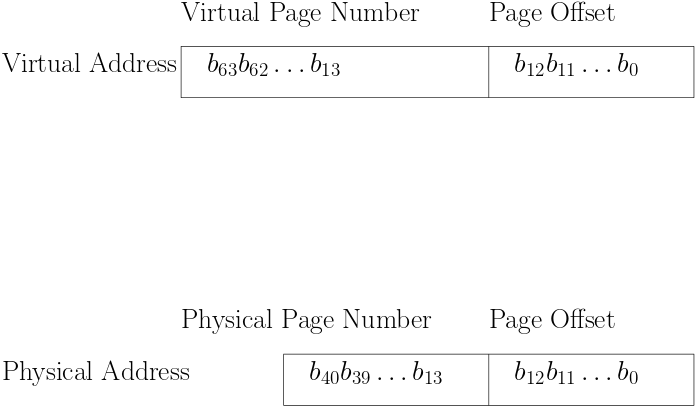
\includegraphics[width=6.0in]{figs/2018s/03_translation.png}}
    \caption{In order to translate the virtual address generated by the CPU to a physical address available on memory unit we use a page table, Translation Lookaside Buffer (TLB), Virtually Indexed Physically Tagged (VIPT) L1 cache, and L2 cache. Use the given page size of $8\text{kB} = 8192 \text{ bits} = 2^{13}$  to determine the 13 bit page offset which is identical for the virtual and physical addresses. The 64 bit virtual address is composed of the 51 bit $\left(b_{63},b_{62},\dots,b_{13}\right)$ virtual page number and the 13 bit $\left(b_{12},b_{11},\dots,b_{0}\right)$ page offset. The 41 bit physical address is composed of the 28 bit $\left(b_{40},b_{39},\dots,b_{13}\right)$ physical page number and the 13 bit $\left(b_{12},b_{11},\dots,b_{0}\right)$ page offset. Use the given Virtually Indexed Physically Tagged (VIPT) 8KB L1 cache for the Translation Lookaside Buffer (TLB) for instructions (iTLB), and the 4MB L2 cache for the TLB for data (dTLB). Using a Virtually Indexed Physically Tagged (VIPT) 8KB L1 cache we can access the cache at the same time as the Translation Lookaside Buffer (TLB) but still get the protection of virtual memory.}
    \label{fig:03_translation_general}
    \end{figure}
    
    \begin{table}
    \centering
    \begin{tabular}{| c c |}
        \hline
        Component & Bit Count \\  
        \hline\hline
        virtual page number & 51\\
        \hline
        physical page number & 28 \\  
        \hline
        page offset & 13\\
        \hline
        TLB index & 0\\
        \hline
        TLB tag & 0\\
        \hline
        cache index & 0\\
        \hline
        cache tag & 0\\
        \hline
    \end{tabular}
    \caption{Component Bit Count}
    \label{table:03_component_bit_count}
    \end{table}

\subsection{Section 2}

\item Given \textbf{A} =
    \begin{bmatrix} 
	1 & 2 & 3 & 4 \\
	-1 & 1 & 3 & 2\\
	2 & 2 & 2 & 4 \\
	\end{bmatrix},
	\textbf{y\textsubscript{1}} =
	\begin{bmatrix} 
	2\\
	-2\\
	4\\
	\end{bmatrix},
	\textbf{y\textsubscript{2}} = 
	\begin{bmatrix} 
	1\\
	1\\
	1\\
	\end{bmatrix}

    \begin{enumerate}
        \item Find a basis for the range space of \textbf{A}, R(\textbf{A})
        \item Find a basis for the null space \textbf{A}, N(\textbf{A})
        \item Find the rank and nullity of \textbf{A}
        \item For the equation \textbf{y\textsubscript{1}} = \textbf{A}\textbf{x\textsubscript{1}}, where \textbf{x\textsubscript{1}} is a $4\times1$ vector, does a solution exist for \textbf{x\textsubscript{1}}?
        \item For the equation \textbf{y\textsubscript{2}} = \textbf{A}\textbf{x\textsubscript{2}}, where \textbf{x\textsubscript{2}} is a $4\times1$ vector, does a solution exist for \textbf{x\textsubscript{2}}?
        \item If a solution \textbf{x\textsubscript{1}} and/or \textbf{x\textsubscript{2}} exist in parts (d) and (e), find \underline{all} solutions.
    \end{enumerate}

\item For the system \textbf{A} =
    \begin{bmatrix} 
	-1 & 8\\
	0.5 & -1\\
	\end{bmatrix},
	\textbf{b} =
	\begin{bmatrix} 
	1\\
	0.5\\
	\end{bmatrix},
	\textbf{c} = 
	\begin{bmatrix} 
	-1\\
	1\\
	\end{bmatrix}
	
	\begin{enumerate}
	    \item Design a state observer;
	    \item Using the state estimates from part a), find an appropriate state feedback such that the system will have a purely oscillatory response with a natural frequency of oscillation $\omega_n = 2$ radians/second.
	\end{enumerate}
	
\item Consider a system with a transfer function 
$$\mathrm{G}(s)=\frac{(s-2)(s-5)}{(s+1)(s-3)(s+4)}$$
Is it possible, using \underline{state feedback} to change it to

    \begin{enumerate}
        \item $\mathrm{G}(s)=\frac{(s-5)}{(s+1)(s+4)}$?
        \item $\mathrm{G}(s)=\frac{s-5}{(s+1)(s+3)(s+4)}$?
    \end{enumerate}
    
If yes, do it. Are the resulting systems controllable? observable? If no, explain why not.

\subsection{Section 3 Communications \& Networks and Signal \& Image Processing, Systems \& Controls}

\item A binary source generates a sequence of symbols with probabilities p and 1-p, respectively. Given the first symbol in the sequence, the source continues to generate symbols until the opposite symbol is generated. Let X denote the length of the sequence, including the first symbol.

    \begin{enumerate}
        \item Find the probability mass function of X.
        \item Find the expected value of X.
    \end{enumerate}
    
\item Messages arriving at a central office switch are exponentially distributed in length, with average length 800 bits and average arrival rate of 16 messages per second. The switch has an infinite buffer and is served by a 64 kilobit per second transmission circuit.

    \begin{enumerate}
        \item Determine the traffic intensity for the switch in Erlangs.
        \item Determine the probability distribution of the number of messages in the buffer.
        \item Determine the average waiting time of a message in the buffer in seconds.
        \item Determine the total average time a message spends in the system, including the waiting time and the service time.
    \end{enumerate}

\item Let $\{\mathrm{Xn}: \mathrm{n}=1,2 \ldots\}$ be an infinite sequence of independent binary random variables with sample values \{0,1) and P\{X n=0\} = 2/3. Let $\text{Yn}=\sum_{\text{i=1}}^{\text{n}} \text{Xi}$ be a random process defined by Xn.

    \begin{enumerate}
        \item For n=5, determine all sample functions of the random process.
        \item Determine the probability mass function of Yn.
        \item Find the expected value and variance of Yn.
        \item Find the autocorrelation function of Yn, $\mathrm{R}\{\mathrm{Y}(\mathrm{n}, \mathrm{n}+\mathrm{k})\}=\mathrm{E}\{\mathrm{Yn} \mathrm{Yn}+\mathrm{k}\}$
    \end{enumerate}
    
\subsection{Section 4 Electromagnetics, Radiation Systems \& Microwave Engineering}

\item The magnetic field of a particular mode in a parallel-plate air waveguide with a plate separation of 2.5 cm is given by
$$H_{z}(x, y)=C e^{-j 640 \pi x / 3} \cos (160 \pi y)$$
where x and y are both in meters.
    
    \begin{enumerate}
        \item Is this a TE\textsubscript{n} or TM\textsubscript{n} mode? What is n? Is it a propagating or non-propagating mode?
        \item What is the operating frequency?
        \item Find the corresponding electric field.
    \end{enumerate}
    
\item An electromagnetic field in free space, $\mu_{0}=4 \pi \times 10^{-7}$ henry/meter, $\varepsilon_0 = 8.85 \times 10^{-12}$ farads/meter, is specified as by the vector phasor 

$$\underline{E}(\underline{r})=\underline{E}_{0} \varepsilon^{-j \underline{k} \underline{g} \underline{r}}$$

where $\underline{E}_{0}=\hat{x}$ the unit vector in the x direction of a rectangular coordinate system (x,y,z).

$$\begin{aligned}
&\underline{r}=x \hat{x}+y \hat{y}+z \hat{z} \\
&\underline{k}=-j \hat{y}+2 \hat{z}
\end{aligned}$$

    \begin{enumerate}
        \item What is the frequency f of the electromagnetic field (Hz)?
        \item Describe the equi-phase surfaces of the field. Write a general equation for the equi-phase surfaces.
        \item Describe the constant magnitude-of-field surfaces. Write a general equation for these equal-magnitude surfaces.
        \item Evaluate the average power as a function of position.
    \end{enumerate}

\item A plane wave is incident in the interface between two dielectrics $\varepsilon_1$ and $\varepsilon_2$, $\varepsilon_1 > \varepsilon_2$ as shown in figure \ref{fig:12q_a}.

\begin{figure}
\centering\fbox{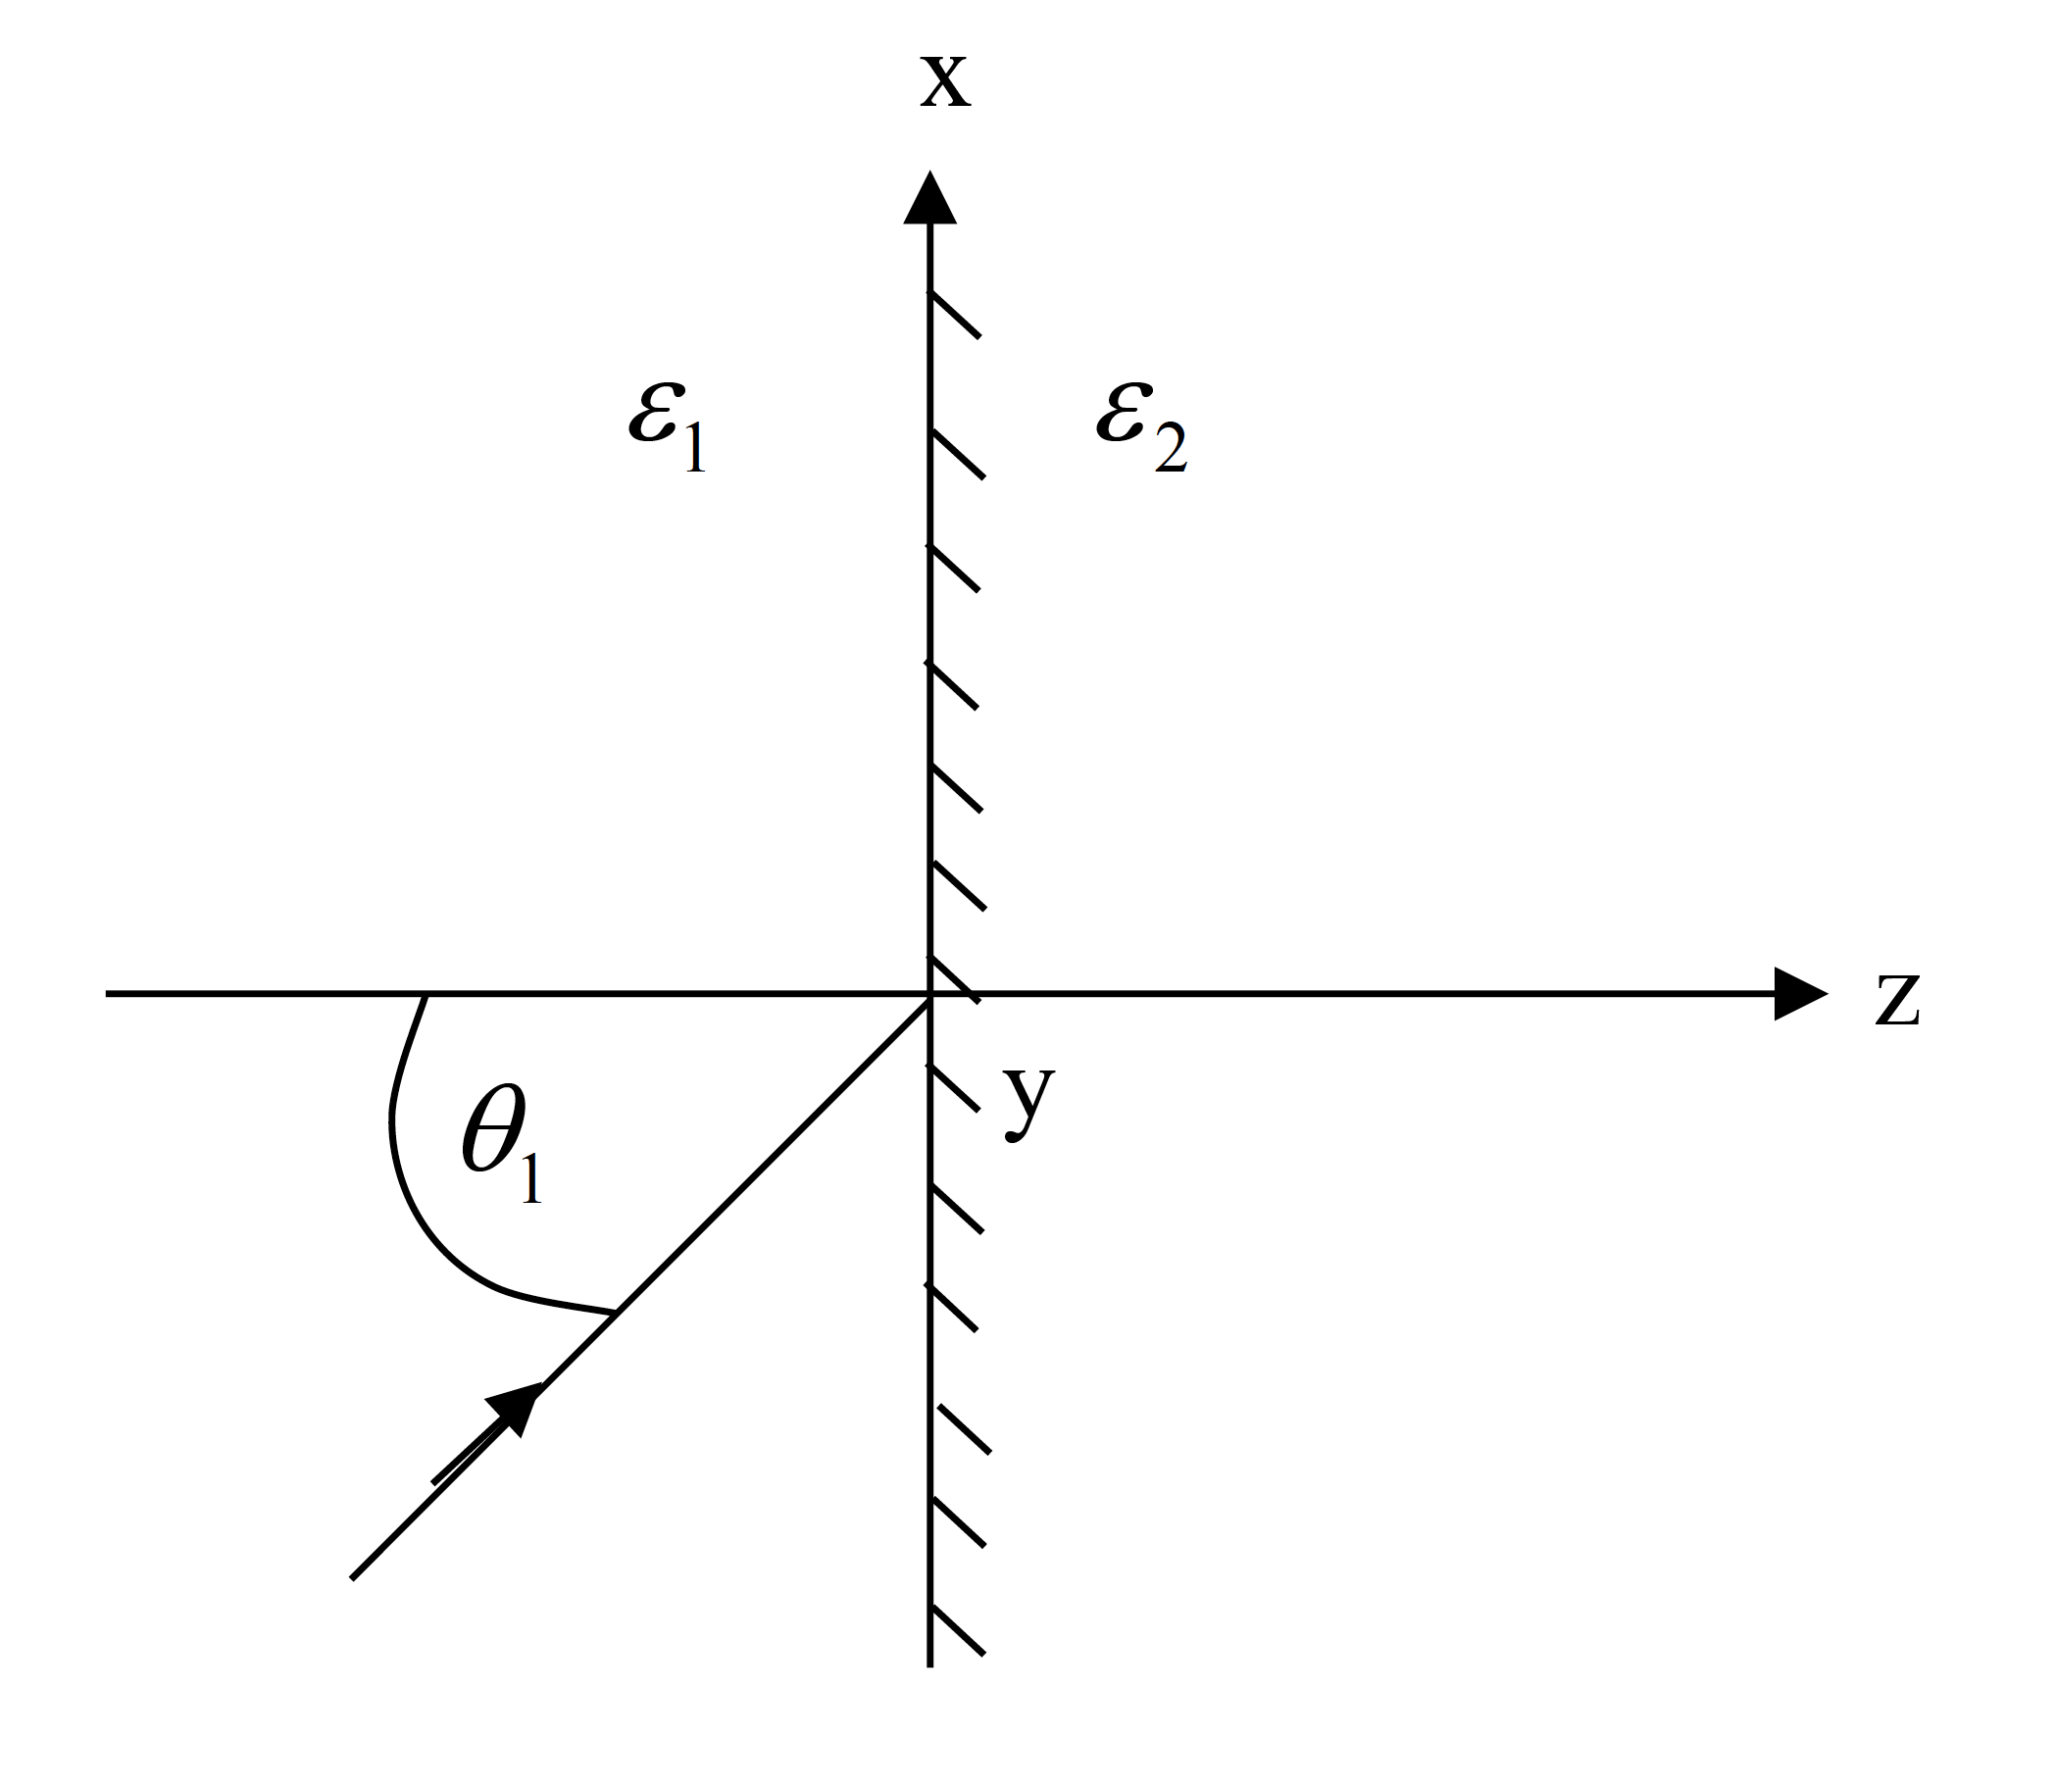
\includegraphics[width=2.0in]{figs/2018s/12q_a.png}}
\caption{Plane wave incident incident in the interface between two dielectrics}
\label{fig:12q_a}
\end{figure}

    \begin{enumerate}
        \item Find the angle $\theta_{1c}$ such that all waves incident with $\theta_1 > \theta_{1c}$ are "totally reflected".
        \item For $\theta_1 > \theta_{1c}$, describe the field (if any) in the region $z > 0$ in the $\varepsilon_2$ dielectric.
        \item If \underline{$E$} is perpendicular to the plane of the incidence, $\underline{E} = E_y \hat{y}$, find the phase of the reflection coefficient.
    \end{enumerate}

\subsection{Section 5} 

\item In the following:

    \begin{enumerate}
        \item Find the Fourier transform of 
        $$x(t)=\frac{\sin (\pi 2 B t)}{\pi 2 B t} \cos \left(2 \pi f_{c} t\right)$$
        where $f_{c}>2 B>0$.
        \item Find the Hilbert transform $\hat{x}(t) \text { of } x(t)$.
        \item Find the analytic signal $\psi(t) \text { of } x(t)$.
        \item Find the complex envelope $\gamma(t) \text { of } x(t)$.
    \end{enumerate}
    
\item Assume that $x[n]$ is a real-valued discrete-time signal and $h[n]$ is a real-valud impulse response of linear time-invariant discrete-time system. Let $y_{1}[n]=x[n] \star h[n]$ represent filtering the signal in the forward direction, where $\star$ stands for convolution. Now filter $y_{1}[n]$ backward to obtain $y_{2}[n]=y_{1}[-n] \star h[n]$. The output is then given by reversing $y_{2}[n]$ to obtain $y[n]=y_{2}[-n]$.

    \begin{enumerate}
        \item Show that this set of operation is equivalently represented by a filter with impulse response $h_{o}[n]$ as $y[n]=x[n] \star h_{o}[n]$ and express $h_{o}[n]$ in terms of $h[n]$.
        \item Show that $h_{o}[n]$ is an even signal and find the phase response of a system having impulse response $h_{o}[n]$. Is the system causal?
        \item Let $H(z)$ and $H_{o}(z)$ be z-transforms of $h[n]$ and $h_{o}[n]$, respectively, and that $h[n]$ is causal. If $H(z)=1 /\left(1-0.9 z^{-1}\right)$ find $H_{o}(z)$, the region of convergence of $H_{o}(z)$, and $h_{o}[n]$.
        \item Repeat (c) if $H(z)=1-0.9 z^{-1}$.
    \end{enumerate}
    
\item Solve the differential equation
    $$y^{\prime \prime}(t)+2 y^{\prime}(t)+y(t)=u(t-1)$$
for $t \geq 0$ using the Laplace transform. $u(t)$ is the unit step function and the initial conditions are $y\left(0^{-}\right)=y^{\prime}\left(0^{-}\right)=1$.

\subsection{Section 6 Electronics, Photonics \& MEMS}

\item Provide clear explanations to the following questions:

    \begin{enumerate}
        \item Using band-theory and energy-related arguments, explain why a metal conducts, an insulator blocks current, and a semiconductor conducts current only under certain situations.
        \item A PN junction is used as a photodetector. Assume that light is shining on all parts of the diode equally. Which part of the photodiode is most critical for photo detection and why? In this application, should the devices be under forward or reverse bias?
        \item After repeated operations of a PMOS MOSFET, hole-type interface traps are formed in the Si-SiO2 interface, does this process increase or decrease the threshold voltage? Draw the band-diagram and the sub-threshold IV curve to illustrate your answer.
    \end{enumerate}

\item MOS Capacitor

    \begin{enumerate}
        \item Draw the band diagram of a MOS system where the "metal" work function $\Phi_{\mathrm{M}}$ is larger than the silicon work function $\Phi_{\mathrm{S}}$. Assume that there are no applied voltages at the p-type substrate (doping $\mathrm{N}_{\mathrm{A}}$) and the gate. On the diagram clearly label the following parameters and functions: electron affinity in the semiconductor $\chi_{\mathrm{Sc}}$, the Fermi level $\mathrm{E}_{\mathrm{F}}$, the conduction and valance band edges $\mathrm{E}_{\mathrm{c}}$ and $\mathrm{E}_{\mathrm{V}}$, the band-gap $\mathrm{E}_{\mathrm{g}}$, the mid-gap $\mathrm{E}_{i}$, the thickness of the oxide $\mathrm{t}_{\mathrm{ox}}$, the potential drop in the oxide $\phi_{\mathrm{ox}}$, and the potential drop in the semiconductor $\phi(\mathrm{x})$
        \item For this device, what is the most likely outcome when no voltages are applied: inversion or accumulation? Why?
        \item Poly-Silicon Gate Depletion (refer to Figure \ref{fig:17q_a}): Assume the voltage $\mathrm{V}_{\mathrm{ox}} = \qty{1}{\volt}$ across a $\qty{2}{\nano\meter}$ thin \ch{SiO2} oxide. The $\mathrm{P}^{+}$ poly gate doping is $\mathrm{N}_{\text {poly }}=1 \times 10^{19} \mathrm{~cm}^{-3}$ and the substrate is n-doped with $\mathrm{N}_{\mathrm{D}}=10^{17} \mathrm{~cm}^{-3}$. Find the poly depletion width, $\mathrm{W}_{\mathrm{dep }}$.
    \end{enumerate}
    
\begin{figure}
    \centering\fbox{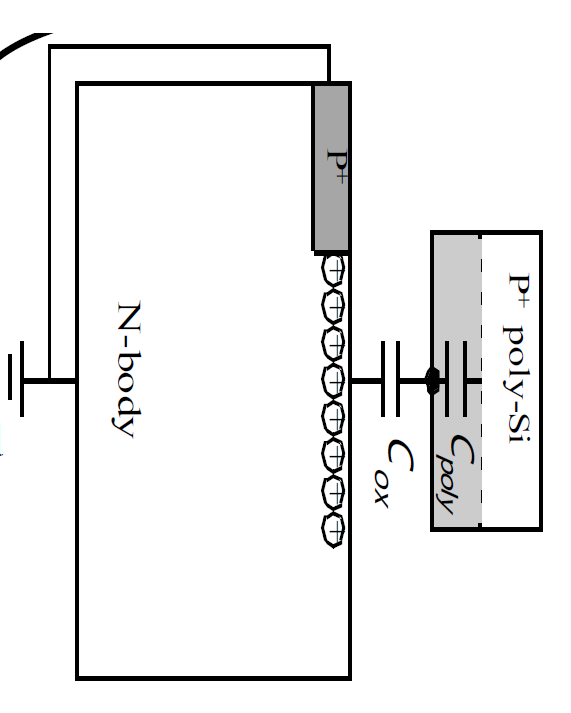
\includegraphics[width=3.0in]{figs/2018s/17q_a.png}}
    \caption{Schematic of the poly depletion capacitances upon gating this MOS capacitor. $\mathrm{T}=300\mathrm{K}$. Gate and body are Silicon. The gate ocide is \ch{SiO2}, $\mathrm{t}_{\mathrm{ox}} = 2 \mathrm{~nm}$}
    \label{fig:17q_a}
\end{figure}

\item Basic \textit{pn}-junction operation.\\

Consider the ideal so-called "long-base" abrupt \textit{pn}-junction silicon diode that has a uniform cross section and constant doping on both sides of the \textit{pn}-junction. The diode is doped as follows: $\mathrm{N}_{\mathrm{a}}=8.0 \times 10^{16} \mathrm{~cm}^{-3}$ \textit{p}-type and $\mathrm{N}_{\mathrm{d}}=1 \mathrm{x} 10^{16} \mathrm{~cm}^{-3}$ \textit{n}-type. For this material, the minority-carrier lifetimes are: $\tau_{\mathrm{n}}=4 \times 10^{-6} \mathrm{~s}$ and $\tau_{\mathrm{p}}=1 \times 10^{-6} \mathrm{~s}$, respectively. You may assume that the effects within the space-charge region are negligible and that the minority carriers flow only by diffusion in the charge neutral regions.

    \begin{enumerate}
        \item Draw/sketch the band-diagram for this system. Also, plot the electrostatic potential, the net charge density and the and the corresponding electric field.
        \item Determine the value of the built-in potential across the \textit{pn}-junction.
        \item Calculate the density of the minority carriers at the edge of the space-charge region for a forward bias of 0.3V.
        \item Under bias condition, calculate and plot the minority and majority carrier currents as a function of distance from the junction.
    \end{enumerate}

\subsection{Section 7}
	
\item Answer the following questions about LANs (wired and wireless):

    \begin{enumerate}
        \item Describe (through some pseudo code and sufficient explanation) CSMA/CD and Binary Exponential Backoff as used in IEEE 802.3 Ethernet.
        \item Describe CSMA/CA (through some pseudo code and sufficient explanation) as used in IEEE 802.11 WiFi.
    \end{enumerate}
    
\item M terminals are attached by a dedicated pair of lines to a hub in a star topology (Figure \ref{fig:20q_a}). The distance from each terminal to the hub is d meters, the speed of the transmission lines is R bits/second, all frames are f length 12,500 Bytes, and the signal propagates on the line at speed of $2.5^{*} 10^{8}$ meters/second. For M=6 terminals, d=25 meters and R = 10Gbps, what is the maximum network throughput achievable when the hub is implementing slotted ALOHA?

\begin{figure}
\centering\fbox{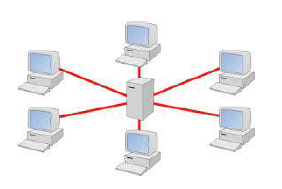
\includegraphics[width=3.0in]{figs/2018s/20q_a.png}}
\caption{Star Topology}
\label{fig:20q_a}
\end{figure}

\item Consider a data link layer with the following parameters: Frame transmission time at the sender is $\mathrm{t}_\mathrm{f}=20$ microseconds. ACK or NAK transmission time at the receiver is $\mathrm{t}_\mathrm{ack} = 10$ microseconds. Link propagation delay on both directions is $\mathrm{t}_{\mathrm{prop}} = 25$ microseconds. Suppose frame processing time at both sender and receiver is negligible, i.e., $\mathrm{t}_{\mathrm{prop}] = 0$. Finally, overall round-trip probability of frame error on the link is $r=0.04$. 

    \begin{enumerate}
        \item Assume that for the Stop-and-wait ARQ scheme, the TIMEOUT at the sender is chosen optimally. What is the resulting throughput (frames/second)?
        \item  In the Go-Back-N ARQ scheme, if the link is error free, what is the minimum window size $N$ that is able to keep the link busy?
        \item Choose window size in Part b and now consider the link error probability $r=0.04$. What the throughput (frames/second) of the Go-Back-N ARQ scheme?
    \end{enumerate}

\subsection{Section 8 Electrical Power \& Energy}

\item A three-phase 250MVA, 20kV, 60Hz salient pole synchronous machine has parameters Xd = 1.1 pu, Xq = 0.6 pu and Ra~0. The machine delivers 230MW at 0.9 lagging power factor to an infinite busbar. Calculate the excitation voltage and power angle. Draw the phasor diagram. (Hint: use per unit values and give your answers in pu).

\item A wind turbine is to be designed with an electrical power output of 7.0MW. The rated upwind free wind speed is 13 m/s. Determine the length of the rotor blades and the height of the supporting tower in meters and the rotational speed of the rotor in rev/min if the tip-speed ratio whose value as 7.0 determines the maximum Power Coefficient of 0.45. Use the density of air as $\num{1.225}\unit{kg/m^3}$

\item A 450MVA, 20kV, 60-Hz round-rotor synchronous generator has an Inertia constant H = 5s. Displayed on the axes in Figure \ref{fig:24q_a} are Torque/Angle characteristics for various faults occurring on a double circuit transmission line when connected between a synchronous generator and an infinite busbar. Using the Equal Area Criterion, determine the critical switching times for both a $3 \varphi$ fault and a Line to Line fault when the input and torque from the turbine is 1.0 pu as shown in the diagram.

\begin{figure}
\centering\fbox{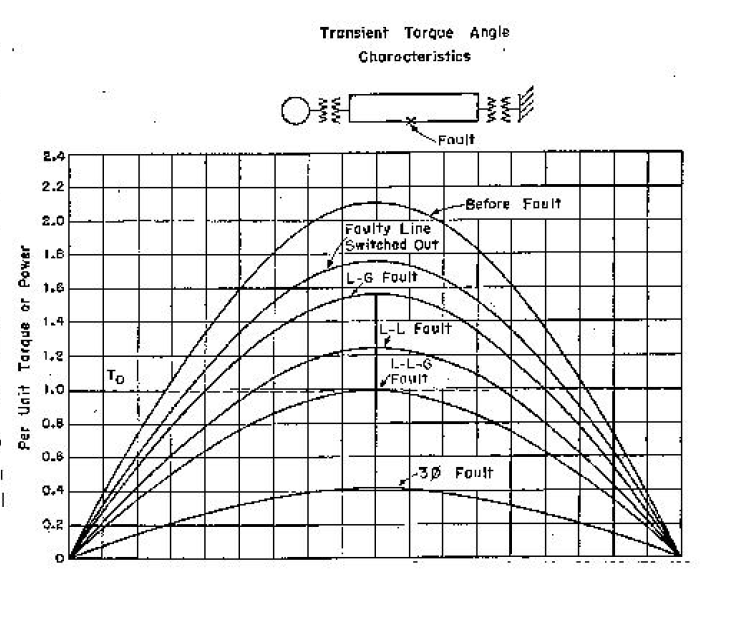
\includegraphics[width=4.0in]{figs/2018s/24q_a.png}}
\caption{Transient Torque Angle}
\label{fig:24q_a}
\end{figure}

\end{enumerate}
\end{document}